\section{\textit{use-case}}
I diagrammi \textit{UML} non sono altro che grafi, utili per rappresentare, grazie alla loro semplicità, - tramite attori e \textit{use-case} - delle specifiche di un progetto non rappresentabili tramite i diagrammi \textit{ER}. \\
I nodi di questo grafo, come accennato, rappresentano attori e \textit{use-case}; gli archi, invece, rappresentano la possibilità di un attore di invocare uno \textit{use-case}. Il nome dell'associazione (arco) è opzionale. \\
In sostanza, questi diagrammi modellano la possibilità di accesso di un attore alla funzionalità di uno use-case.

\subsection{Associazioni tra \textit{use-case}}
È possibile collegare \textit{use-case} tra di loro con archi in una sorta di ereditarietà.
\begin{itemize}
    \item \textit{include}: \textit{A} include \textit{B}. Si presuppone che alcune funzioni di \textit{A} richiedano funzioni di \textit{B}.
    \item \textit{extends}: \textit{A} estende \textit{B}. \textit{A} necessita di alcune funzioni di \textit{B}, o di reimplementarle.
\end{itemize}
\begin{center}
    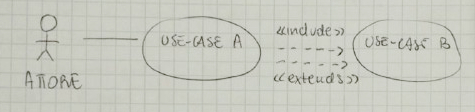
\includegraphics[width=.7\textwidth]{res/uml-usecase1.jpg} \hfill
\end{center}
\newpage

\subsection{Associazioni tra attori}
Le associazioni tra attori ricordano le relazioni \textit{is-a}: in questo caso \textit{A} è un \textit{caso particolare} di \textit{B}.
\begin{center}
    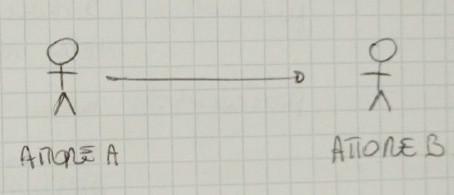
\includegraphics[width=.7\textwidth]{res/uml-usecase2.jpg} \hfill
\end{center}

\section{Specifiche \textit{use-case}}
La struttura delle specifiche \textit{use-case} è formata dai seguenti parametri:
\begin{enumerate}
    \item \textit{operazione}(\textit{arg1}: \textit{dom1}, \ldots:\ldots, \textit{argN}:\textit{domN}): \textit{domR}
    \begin{itemize}
        \item \textit{operazione} è il nome della operazione, della procedura, descritta dalla specifica;
        \item \textit{argN} è un'istanza di (dominio) \textit{domN} presa in input dalla specifica;
        \item \textit{domR} è il dominio del valore ritornato in output dalla specifica.
    \end{itemize}
    \item \textit{precondizioni}: viene esplicitato sottoforma di linguaggio naturale la precondizione (o le precondizioni) che devono essere soddisfatte perché possa essere applicata la data specifica. Rappresentano le condizioni sugli argomenti e sul livello estensionale del sistema, che devono valere all'avvio dell'operazione affinchè il suo comportamento sia definito;
    \item \textit{postcondizioni}: viene esplicitato sottoforma di linguaggio naturale l'operazione che viene applicata dalla specifica. Rappresentano le condizioni sul livello estensionale del sistema, che devono valere al termine dell'operazione (nel caso in cui questa faccia side-effect).
\end{enumerate}

\paragraph{Esempio 1}
\begin{itemize}
    \item \textit{mediaVoti}(s : Studente): reale in [18,31]
    \item \textit{precondizioni}: l'istanza s deve essere coinvolta in almeno 1 istanza della relazione Esame.
    \item \textit{postcondizioni}: result è la somma dei valori dell'attributo Voto di tutte le istanze di Esame - definite nel livello estensionale - nelle quali l'istanza s è coinvolta.
\end{itemize}
\paragraph{Esempio 2}
Caso relativo alla use-case: \textit{Esame}
\begin{itemize}
    \item \textit{verbalizzaEsame}(s : Studente, c : Corso, v : [18,31])
    \item \textit{precondizioni}: s non è coinvolta in nessuna istanza della relazione Esame con c.
	\item \textit{postcondizioni}: viene creata l'istanza della relazione Esame tra s e c con attributo Voto valorizzato a v.
\end{itemize}

\section{Efficienza e problemi del linguaggio UML}
Nonostante la sua estrema semplicità - che permette di scrivere specifiche complesse senza grandi difficoltà -, è proprio questo la causa di diversi problemi che potrebbe presentare il linuaggio \textit{UML}:
\begin{itemize}
    \item potenzialmente ambiguo;
    \item potenzialmente emissivo;
    \item contraddittorio;
    \item poco leggibile.
\end{itemize}